\documentclass[11pt]{article}
\usepackage[letterpaper,margin=1in]{geometry}
\usepackage{amsmath,amssymb,amsthm}
\usepackage{graphicx}
\usepackage{booktabs}
\usepackage{caption}
\usepackage{subcaption}
\usepackage{enumitem}
\usepackage{titlesec}
\usepackage{fancyhdr}
\usepackage{placeins}
\usepackage{float}
\usepackage{xcolor}
\PassOptionsToPackage{hyphens}{url}
\usepackage[hidelinks]{hyperref}
\usepackage{xurl}
\setlength{\parskip}{0.4em}
\setlength{\parindent}{0pt}
\setlength{\emergencystretch}{2em}
\titleformat{\section}{\large\bfseries}{\thesection.}{0.6em}{}
\titlespacing*{\section}{0pt}{1.4em}{0.5em}
\titleformat{\subsection}{\normalsize\bfseries}{\thesubsection}{0.5em}{}
\titlespacing*{\subsection}{0pt}{1.0em}{0.3em}
\captionsetup{font=small,labelfont=bf,labelsep=period,skip=6pt}
\setlist[itemize]{leftmargin=1.3em,itemsep=2pt,topsep=3pt,parsep=0pt}
\setlist[enumerate]{leftmargin=1.6em,itemsep=2pt,topsep=3pt,parsep=0pt}
\pagestyle{fancy}
\fancyhf{}
\fancyhead[L]{\small CS 6362: Advanced Machine Learning}
\fancyhead[R]{\small Assignment 2 \,\textbar\, Bibek Dhungana}
\fancyfoot[C]{\small\thepage}
\renewcommand{\headrulewidth}{0.4pt}
\newcommand{\code}[1]{\texttt{#1}}
\newcommand{\repo}[1]{\nolinkurl{#1}}   % repository names, may break at / and -
\newcommand{\E}{\mathbb{E}}
\newcommand{\R}{\mathbb{R}}
\newcommand{\KL}[2]{D_{\mathrm{KL}}\!\left(#1\,\|\,#2\right)}
\newcommand{\TODO}[1]{\textcolor{red}{[#1]}}
\newtheorem{theorem}{Theorem}

\begin{document}
\begin{center}
  {\LARGE\bfseries Paper 2: On Large-Batch Training for Deep Learning:\\[2pt] Generalization Gap and Sharp Minima}\\[5pt]
  {\large Keskar, Mudigere, Nocedal, Smelyanskiy, Tang (ICLR 2017)}\\[4pt]
  Bibek Dhungana \quad\textbar\quad CS 6362 Assignment 2 \quad\textbar\quad \today
\end{center}

\section{Problem statement and summary}

\subsection{Setup}
Training minimizes the average loss over the training set,
\[
  \min_{x\in\R^n} f(x)=\frac1M\sum_{i=1}^M f_i(x),
\]
where, in the paper's notation, $x$ is the vector of all $n$ weights, $M$ is the number of training examples and $f_i(x)$ is the cross-entropy loss on example $i$. A mini-batch method picks a random subset $B_k$ at step $k$ and steps against its average gradient,
\[
  x_{k+1}=x_k-\alpha_k\,\frac{1}{|B_k|}\sum_{i\in B_k}\nabla f_i(x_k).
\]
The paper compares a small batch (SB, $|B_k|=256$) with a large batch (LB, $|B_k|=10\%$ of the training set, i.e.\ 6{,}000 on MNIST and 5{,}000 on CIFAR-10), with ADAM in both cases and everything else equal.

Both reach about the same training accuracy, but LB tests worse (Table~2 of the paper): 98.03\% against 97.81\% on F1, 80.04\% against 77.26\% on C1, and 89.24\% against 87.26\% on C2. This is the \emph{generalization gap}. It is not ordinary overfitting: the LB test accuracy does not rise and then fall, so early stopping would not fix it.

\subsection{The claim: large batches end in sharp minima}
A minimizer is \emph{sharp} if the loss rises quickly when the weights move a little, and \emph{flat} if it stays low in a wide neighborhood; in terms of the Hessian $\nabla^2 f$, sharp means large eigenvalues. The intuition for why flat is better: the test loss looks like the training loss shifted a little. If the training loss is $\tfrac{c}{2}x^2$ and the test loss is the same parabola shifted by 0.1, the test loss at the training minimum is $\tfrac{c}{2}\,0.1^2$, which is 0.005 for a flat minimum ($c=1$) and 0.5 for a sharp one ($c=100$).

The paper gives two main kinds of evidence. The first is Figure~3, the one I reproduce. With $x_s^\star$ and $x_\ell^\star$ the SB and LB solutions, it plots the loss along the line through both,
\[
  \phi(\alpha)=f\big(\alpha\,x_\ell^\star+(1-\alpha)\,x_s^\star\big),\qquad \alpha\in[-1,2],
\]
so $\alpha=0$ is the SB solution and $\alpha=1$ the LB solution. In the paper the loss forms a wide bowl around $\alpha=0$ and a narrow notch around $\alpha=1$. The second is a sharpness number (Metric~2.1): the largest relative rise of the loss in a small box around the solution, found with ten L-BFGS-B iterations. The LB values are 10 to 100 times the SB values (Tables 3 and 4).

\subsection{Why the batch size should matter}
The batch gradient is the true gradient plus noise, $g_B=\nabla f(x)+\xi_B$. For a batch of $|B|$ independently drawn examples,
\[
  \operatorname{Cov}(\xi_B)=\frac{1}{|B|}\,\Sigma(x),\qquad \Sigma(x)=\frac1M\sum_{i=1}^M\big(\nabla f_i-\nabla f\big)\big(\nabla f_i-\nabla f\big)^{\!\top},
\]
so going from 256 to 5{,}000 examples divides the noise variance by about 20. The paper's picture is that SB noise kicks the weights out of narrow valleys, so SB only settles in wide ones, while LB behaves like plain gradient descent and stops in the first minimum it reaches.

\subsection{Answers to the questions in the assignment}
\textbf{Which networks and datasets correspond to F1, C1 and C2?} F1 is a fully connected network on MNIST: 784 inputs, five layers of 512 units with batch norm and ReLU, 10 outputs. C1 is a shallow AlexNet-like network on CIFAR-10: two blocks of a $5\times5$ convolution with 64 filters and $3\times3$ max-pooling, then dense layers of 384 and 192 units with dropout, and batch norm on every layer. C2 is a deep VGG-like network on CIFAR-10: stacks of 2, 2, 3, 3, 3 convolutions ($3\times3$) with 64, 128, 256, 512, 512 filters, max-pooling after each stack, and a dense layer of 512 units.

\textbf{What range of $\alpha$ does Figure 3 use, and what is on each axis?} $\alpha$ runs from $-1$ to $2$ on the horizontal axis. The left axis is the cross-entropy loss (blue) and the right axis the classification accuracy in percent (red). Solid lines are the training set, dashed lines the test set.

\textbf{What batch sizes and optimizer define SB and LB?} SB uses 256 examples and LB 10\% of the training set, both with ADAM. The paper gives no ADAM settings (the released code uses the defaults). Each experiment is repeated five times from different starting points, and the networks are trained ``until the loss function ceased to improve''.

\section{Reproduction of Figure 3 (F1, C1, C2)}

\subsection{LLM, conversation and code}
\begin{itemize}
  \item \textbf{LLM:} ChatGPT (GPT-5.6) for the main conversation. I also asked Claude and Gemini some side questions to understand concepts related to the paper.
  \item \textbf{Shared conversation}:\newline \url{https://chatgpt.com/share/e/6ad7087b-6704-83e8-9168-a7a5151d61f2}
  \item \textbf{Code:} folder \repo{paper2:Generalization-Gap-and-Sharp-Minima/code} of\newline \url{https://github.com/dhunganabibek/reading-and-reproducing-papers}. The notebook \code{reproduce\_fig3.ipynb} redraws the required figure and prints the saved measurements. Training logs, interpolation results and weight-distance summaries are included; the large weight files are regenerated by \code{run\_all.sh}.
\end{itemize}

\subsection{Setup and choices}

\textbf{Batch-norm statistics at interpolated weights.} The running means and variances of batch norm are measured during training, so there is no value for them between two solutions. I either \emph{re-measure} them by passing the training set through the network at the interpolated weights, or \emph{interpolate} the two stored values with the same $\alpha$ as the weights. The main figure re-measures, because that evaluates the network the interpolated weights actually define, and it avoids mixing statistics from different solutions. It differs from the authors' use of current-batch statistics at evaluation (Section~\ref{sec:phase4}).

\textbf{Shared starting point.} Both runs of a pair start from the same random weights, which controls initialization. Batch size also changes the number of updates per epoch and, for the chunked convolutional runs, the batch-norm statistics.

\begin{table}[htb]\centering\small
  \begin{tabular}{@{}l@{\quad}p{0.76\textwidth}@{}}
    \toprule
    Data & MNIST with pixels in $[0,1]$; CIFAR-10 standardized per color channel; no augmentation\\
    Networks & F1 (1.46M weights), C1 (1.76M), C2 (15.0M), as in Appendix B of the paper\\
    Optimizer & ADAM with PyTorch defaults (learning rate $10^{-3}$, $\beta=(0.9,0.999)$) for both\\
    Batch sizes & SB 256; LB 6{,}000 (MNIST) and 5{,}000 (CIFAR-10)\\
    Training length & 100 epochs for both, as in Figures 2, 4 and 5 of the paper\\
    Interpolation & 61 values of $\alpha$ in $[-1,2]$; loss and accuracy on the full train and test sets; dropout off\\
    Seeds & one pair per network; three pairs for F1\\
    \bottomrule
  \end{tabular}
  \caption{Setup of my runs.}
\end{table}

\textbf{Training length.} In 100 epochs SB makes about 19{,}500 updates on CIFAR-10 and LB only 1{,}000.

\begin{figure}[H]\centering
  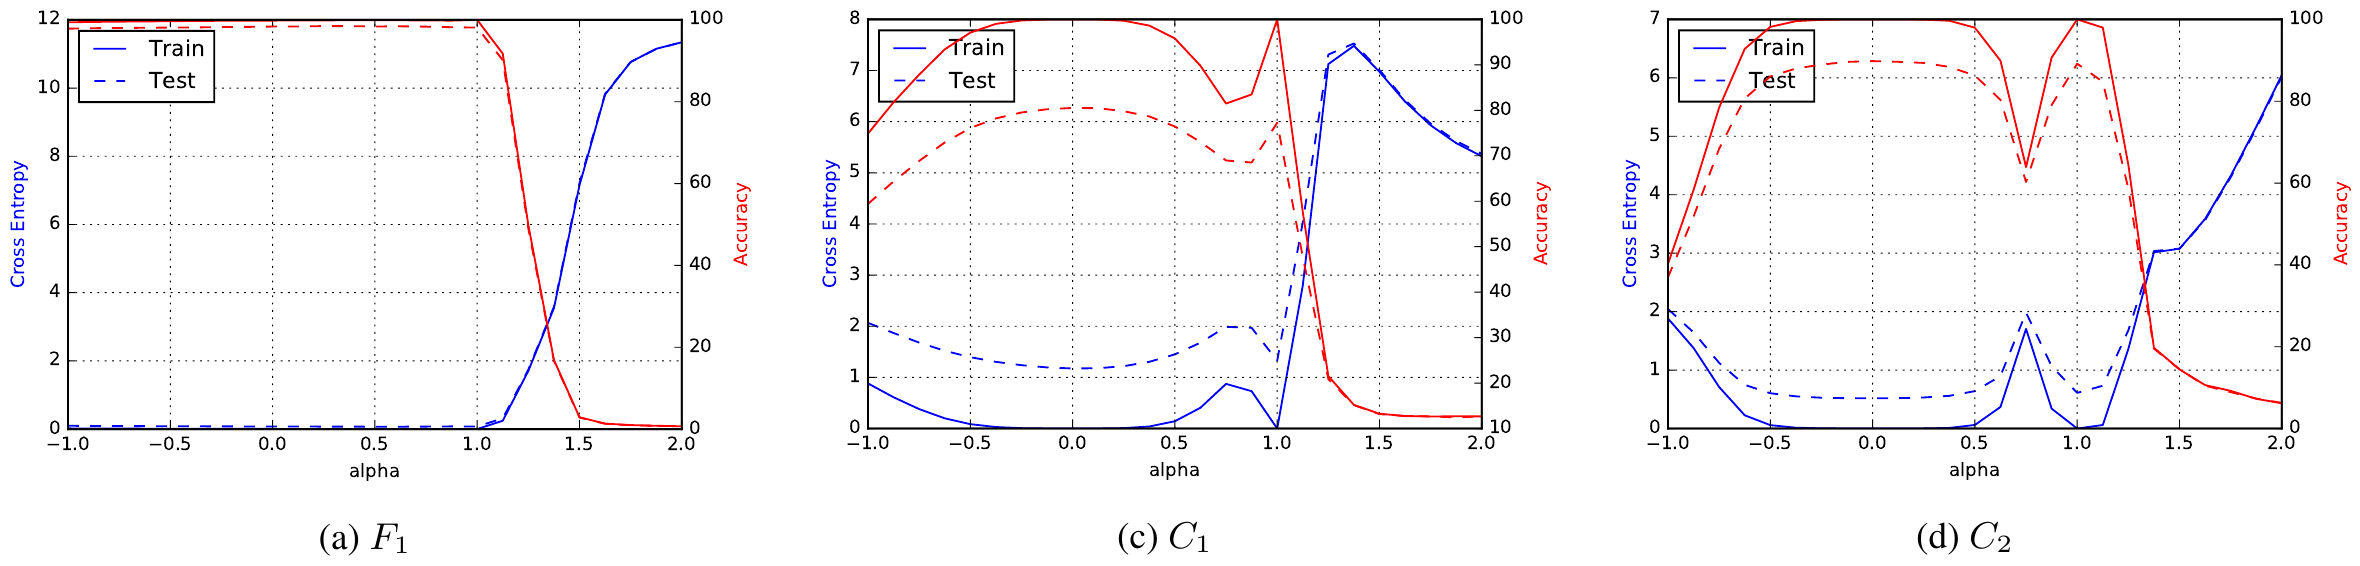
\includegraphics[width=0.84\textwidth]{figures/original_fig3_f1c1c2.png}\\[5pt]
  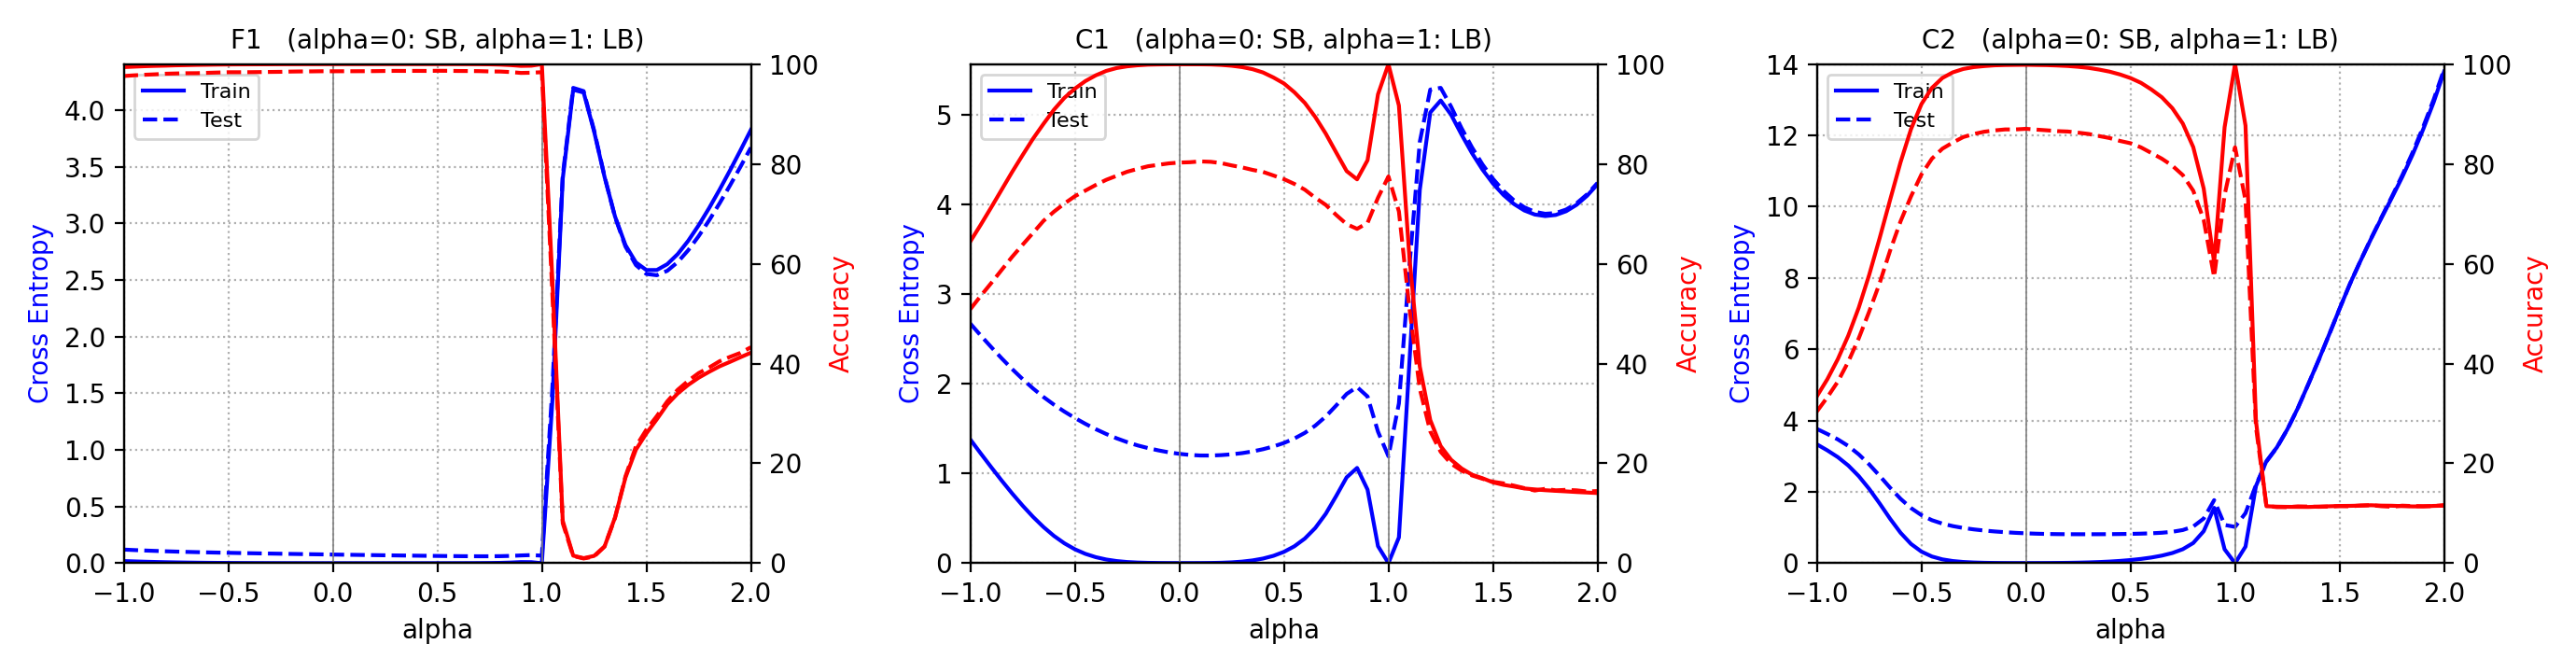
\includegraphics[width=0.98\textwidth]{figures/fig3_reproduced_bn-recompute.png}
  \caption{Top: panels F1, C1, C2 of Figure 3 of the paper. Bottom: my reproduction, with batch-norm statistics re-measured at every $\alpha$. Blue is the cross entropy and red the accuracy; solid is train, dashed is test.}
  \label{fig:fig3}
\end{figure}

\subsection{Results}\label{sec:results}
Both methods fit the training set and LB tests worse (Table~\ref{tab:acc}). The SB advantage in test accuracy is 0.20 points on F1 (paper: 0.22), 3.4 on C1 (paper: 2.8) and 3.4 on C2 (paper: 2.0). For F1 I trained three pairs, and the gap was 0.20, 0.15 and $-0.01$ points. On this network the gap is about as large as the difference between two runs, so one pair cannot establish it.

\begin{table}[H]\centering\small
  \begin{tabular}{@{}l l cc cc c@{}}
    \toprule
    & & \multicolumn{2}{c}{mine (one pair)} & \multicolumn{2}{c}{paper (mean of 5)} & $\|x_s^\star-x_0\|\,/\,\|x_\ell^\star-x_0\|$\\
    \cmidrule(lr){3-4}\cmidrule(lr){5-6}
    network & method & train & test & train & test & mine\\
    \midrule
    F1 & SB & 100.00 & 98.61 & 99.66 & 98.03 & \\
    & LB & 100.00 & 98.41 & 99.92 & 97.81 & 14.3\\
    \addlinespace
    C1 & SB & 99.94 & 80.06 & 99.89 & 80.04 & \\
    & LB & 99.88 & 76.64 & 99.66 & 77.26 & 4.8\\
    \addlinespace
    C2 & SB & 99.82 & 86.75 & 99.99 & 89.24 & \\
    & LB & 100.00 & 83.32 & 99.99 & 87.26 & 11.3\\
    \bottomrule
  \end{tabular}
  \caption{Accuracy in percent after 100 epochs, and how much farther SB ends from the common starting point $x_0$ than LB (the paper reports 3 to 10).}
  \label{tab:acc}
\end{table}

\textbf{The plots (Figure~\ref{fig:fig3}).} For F1 the loss stays below 0.02 for every $\alpha$ from $-1$ to $1$, as in the paper, and jumps right behind the LB solution. C1 matches the paper's panel: a wide bowl around the SB solution, a bump of 1.1 at $\alpha=0.85$, a narrow notch at the LB solution and a wall behind it. A quarter of the way beyond the SB solution ($\alpha=-0.25$) the C1 training loss is 0.01; a quarter of the way beyond the LB solution ($\alpha=1.25$) it is 5.2. C2 has the same shape, with a bump of 1.6 at $\alpha=0.9$ and 0.02 against 3.8 for the same two steps. So along this line the LB solution sits in a much narrower valley, as in the paper (but see Section~\ref{sec:review}).

\begin{figure}[htbp]\centering
  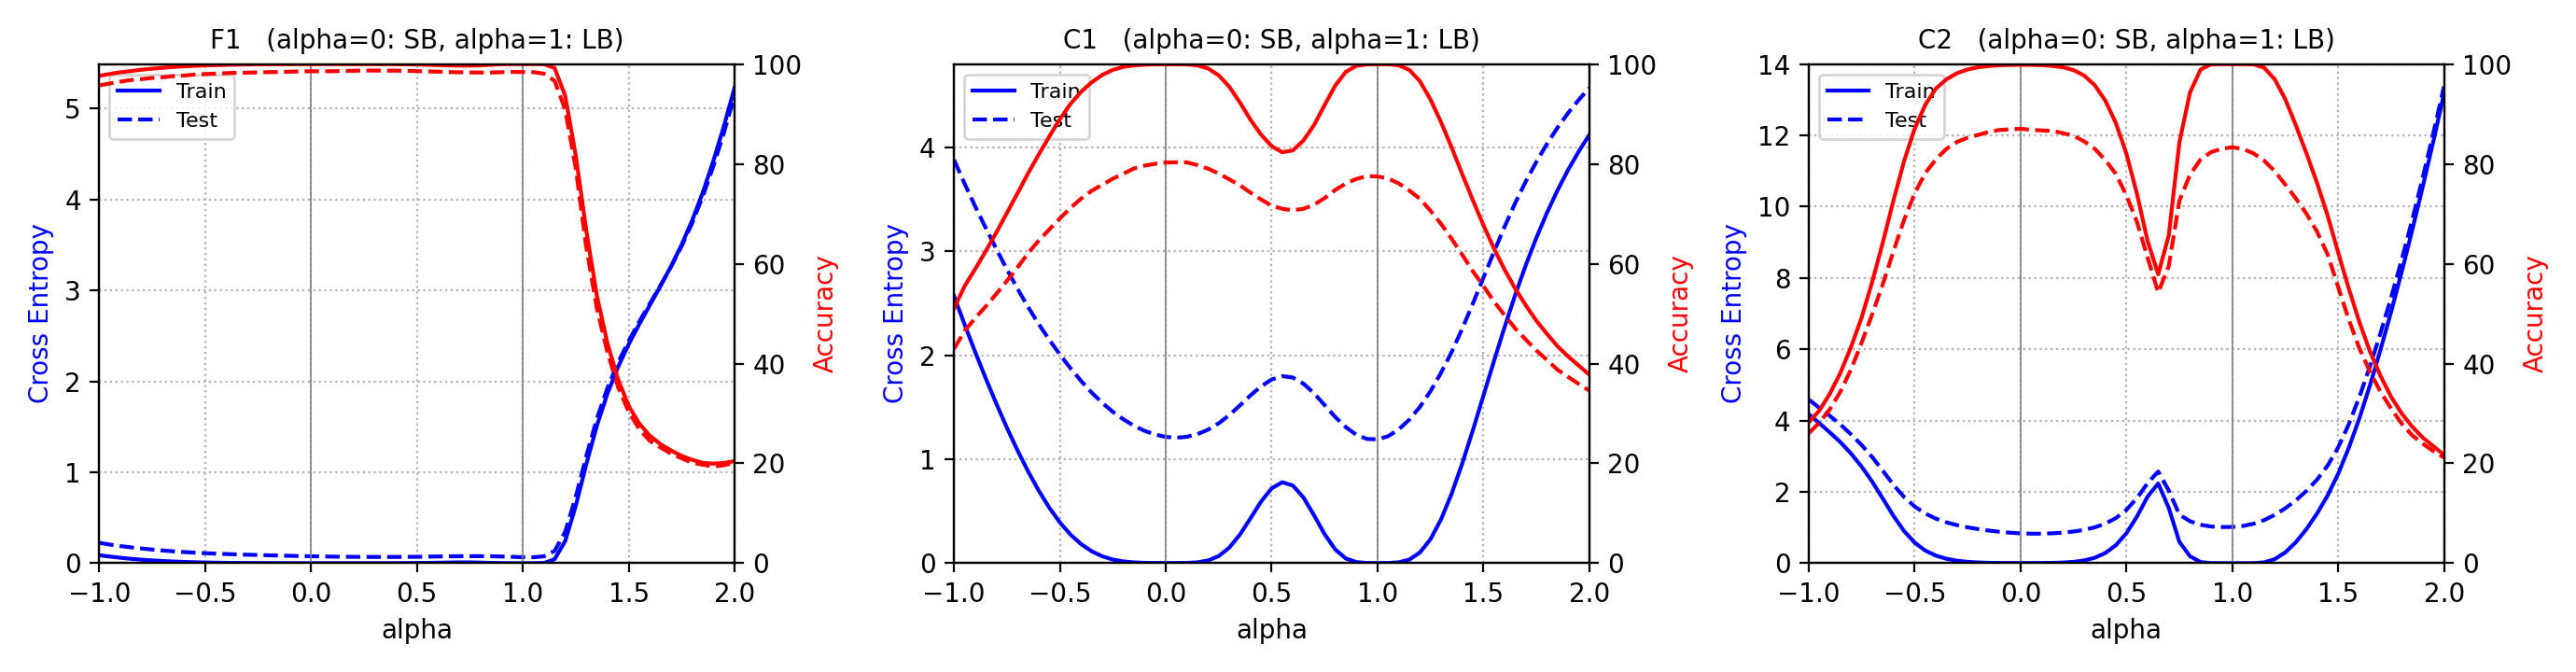
\includegraphics[width=0.98\textwidth]{figures/fig3_reproduced_bn-recompute_norm.png}
  \caption{The same runs with batch-norm statistics re-measured after rescaling every layer that feeds a batch norm to the same norm in both solutions, which approximately preserves the endpoints after recalibration (Section~\ref{sec:review}).}
  \label{fig:variants}
\end{figure}

\textbf{The batch-norm choice matters.} With interpolated statistics the bump in front of the LB solution grows from 1.1 to 7.4 for C1, and F1 gets a bump of 1.4 that the re-measured version does not have. The stored variances of the two networks are very different (in F1 the SB ones are typically 40 to 300 times larger), so mixing them normalizes the mixed network wrongly. That barrier is partly a bookkeeping artifact.

\subsection{Phases 1--3: failures and corrections}
In Phase~1 I gave the LLM the paper PDF and asked for PyTorch code that reproduces panels F1, C1 and C2 of Figure~3. Checking that code against the paper and running it (Phases 2 and 3) turned up these problems:
\begin{itemize}
  \item \textbf{Stopping too early.} ``Until the loss ceased to improve'' was first coded as: stop when the training loss has not improved by 1\% for 10 epochs. One LB epoch is only 10 updates, so the C1 LB run stopped after 76 epochs at 93.5\% training accuracy (paper: 99.66\%). Counting updates instead made LB run for hundreds of epochs while SB stopped after about 60. In the end I used the paper's 100 epochs for both.
  \item \textbf{Wrong C1.} The paper writes C1 as $2\times[64,5,5,2]$ followed by MaxPool(3), where $[a,b,c,d]$ means $a$ filters of size $b\times c$ with stride $d$, so I built stride-2 convolutions. That network has 0.28 million weights and reached only about 70\% test accuracy with SB (paper: 80\%). I suspected the architecture but could not resolve it from the paper; Phase~4 did.
  \item \textbf{Dropout on while re-measuring batch-norm statistics.} My first version re-measured in training mode, which also turns dropout on, so the variances after a dropout layer were too large. Now only the batch-norm layers are in training mode, and the statistics agree with those of the evaluated network to within 1\%.
  \item \textbf{Memory.} A batch of 5{,}000 CIFAR images needs 9~GB of GPU memory in C1 and about 18~GB in C2, and four jobs at once had already crashed the laptop. Large batches are now processed in chunks (2{,}500 images for C1, 1{,}250 for C2) and the gradients added up before the step. There is still one ADAM step per large batch, but this is not the exact full-batch gradient: batch norm sees each chunk, and dropout samples depend on how the forward passes are grouped.
\end{itemize}

\subsection{What did not match, and why}
\textbf{Accuracy of C2.} My C2 is 2.5 to 4 points below the paper for both methods (86.8\% and 83.3\% against 89.2\% and 87.3\%). The released C2 has dropout after most convolutions, which I did not use (Section~\ref{sec:phase4}). That is one possible explanation, but I did not isolate it with an ablation.

\textbf{Size of the gap and distance from the start.} My gaps on C1 and C2 (3.4 points each) are larger than the paper's (2.8 and 2.0), but with one pair per network I cannot tell whether that is real; on F1 the gap moves by 0.2 points from pair to pair. The distance ratio is 14 for F1 and 11 for C2, above the paper's range of 3 to 10; for C1 it is 4.8.

\textbf{The wall in F1.} In the paper's F1 panel the loss rises gradually behind the LB solution; in mine it jumps. After the rescaling in Section~\ref{sec:review} mine looks like the paper's (Figure~\ref{fig:variants}, left). My guess is that the two solutions of the paper's F1 pair differed less in weight scale than mine, but the paper does not report weight norms.

\subsection{Phase 4: comparison with the authors' code}\label{sec:phase4}
After saving the Phase~3 code I read the authors' Keras~1 repository \repo{keskarnitish/large-batch-training}. Because of the crash, only F1 and my first C1 had been trained at that point, both with stopping rules I later dropped; all numbers in this report come from runs made afterwards with the final code.

\textbf{C1 (changed).} In the released code the convolutions have stride 1 and the max-pooling has stride 2, so the dense layer sees $8\times8\times64=4096$ features instead of 256 and the network has 1.76 million weights. With this C1 my SB run reaches 80.06\% test accuracy (paper: 80.04\%). My first reading is kept as \code{C1s2}; it reaches 69.2\% (SB) and 64.3\% (LB).

\textbf{Training length (changed).} The script trains both methods for a fixed number of epochs (20) and the paper's figures use 100, so I replaced my stopping rule by 100 epochs.

\textbf{Batch-norm statistics and starting point (confirmed).} The script interpolates only the trainable weights, and its batch norm uses the statistics of the current batch at test time too (Keras ``mode 2''). My variant instead averages training-batch statistics and uses those fixed values for evaluation. Both avoid interpolating stored statistics, but they are not equivalent, including on the training set because current-batch and averaged statistics differ. The script also saves the initial weights, trains SB, reloads them and trains LB, so a pair shares its starting point as in my runs.

\textbf{C2 (not changed).} The released C2 has dropout after most convolutions, while Appendix~B.4 only describes dropout on the dense layer; I follow the paper. The script also feeds unstandardized inputs in $[0,1]$ and uses 25 values of $\alpha$ where I use 61.

Changes after the Phase~3 snapshot: the C1 architecture, the 100 epochs and re-measured batch-norm statistics in the main figure (because of the released code and the paper's figures); chunked large batches, dropout off while re-measuring statistics and saving the initial weights (my own fixes); and the rescaled variant of the plot used in the review. The final cleanup keeps the recorded runs, saves weight-distance summaries so the notebook works without large weight files, and recomputes interpolation when either trained endpoint changes. New checkpoints also save CPU and device random-number states for continuation after interruption.

\section{Critical review}

\subsection{My review}\label{sec:review}
The paper shows on six networks that large-batch ADAM reaches the same training accuracy as small-batch ADAM but lower test accuracy. It attributes this to large batches converging to sharp minima, and supports the claim with one-dimensional plots between the two solutions, a sharpness number and warm-start experiments.

\textbf{Strengths.} The question matters in practice, since large batches are what makes training on many processors efficient. The experiments are simple and can be rerun on a laptop. The paper separates the observation (the gap) from the proposed cause (sharpness), tests the cause in several ways, and even reports remedies that only partly worked (Appendix~E).

\textbf{Weaknesses.}
\begin{itemize}
  \item \emph{Sharpness is not a property of the function the network computes.} In a ReLU network one can multiply the weights of one layer by 10 and divide those of the next by 10. The function stays exactly the same, but the loss surface around the new weights is stretched in some directions and squeezed in others, so the sharpness changes. Dinh et al.\ (2017, ``Sharp minima can generalize for deep nets'') used this to make any minimum arbitrarily sharp. A number that changes when the function does not cannot by itself explain generalization.
  \item \emph{The two methods do not get the same amount of optimization.} For the same number of epochs LB makes about 20 times fewer updates. Both still fit the training set in my runs, so LB is not under-trained in the obvious sense, but SB ends 5 to 14 times farther from the starting point (Table~\ref{tab:acc}). Later papers closed most of the gap by training LB for more updates with a larger learning rate (Hoffer et al.\ 2017; Goyal et al.\ 2017), so part of the gap is about the training budget, not the batch size as such.
  \item \emph{A straight line is a thin probe.} The plot shows one direction out of millions, and it depends on the distance and scale of the two solutions. In my runs the SB weights are 1.5 to 9 times larger than the LB weights in every layer that feeds a batch norm (for F1 about 70 against 14). Batch norm approximately cancels that scale after its statistics are recalibrated. The cancellation would be exact for a single layer with zero epsilon and consistently scaled statistics; finite epsilon and multilayer recalibration can change predictions. Thus this experiment is a normalization diagnostic, not an exact function-preserving transformation. After that (Figure~\ref{fig:variants}) the LB notch of C1 and C2 widens into a bowl much like the SB one, the F1 wall becomes a gradual slope, and the training loss a quarter of the way beyond the LB solution drops from 3.8--5.2 to 0.2--0.6. The LB solution is still the narrower one (the same step beyond SB costs at most 0.04), but by much less than the standard plot suggests. Li et al.\ (2018, ``Visualizing the loss landscape of neural nets'') later made the same point.
  \item \emph{Batch norm is not discussed.} All networks use it, and the paper does not say which statistics are used between the two solutions; with my two choices the C1 barrier is 1.1 or 7.4.
  \item \emph{One pair out of five.} Figure~3 shows one randomly chosen pair per network and no spread.
\end{itemize}

\textbf{Possible errors and unclear points.}
\begin{itemize}
  \item In the paper's F1 panel the loss is almost zero for all $\alpha$ from $-1$ to $1$ and only rises beyond the LB solution. That is hard to call a ``strikingly sharper'' minimum, as the text does; the LB solution sits at the edge of a wide flat region. My F1 run has the same shape, and its two test accuracies differ by only 0.2 points.
  \item The notation $2\times[64,5,5,2]$ for C1 suggests stride-2 convolutions, but in the released code the stride belongs to the pooling layer.
  \item Appendix~B.4 describes C2 with dropout only on the dense layer, but the released code has dropout after most convolutions too.
  \item The sharpness numbers come from only ten iterations of an inner optimizer; a different budget would give different numbers.
\end{itemize}

\subsection{Comparison with the OpenReview reviews}
\noindent\href{https://openreview.net/forum?id=H1oyRlYgg}{OpenReview discussion and public reviews}.

The reviewers gave 8, 10 and 6, and the paper was accepted. The reviewer who gave 10 saw ``little novelty but valuable empirical evidence'' and had one correctness concern: the first version claimed the sharpness measure was scale invariant, and the authors removed the claim. The reviewer who gave 6 found the paper ``interesting and useful'' and suggested adding scaled Gaussian noise to the large-batch gradients to see whether that recovers the small-batch behavior. A public comment proposed the same test.

My first weakness is the 10-rating reviewer's concern taken one step further: the claim was removed, but the measure still depends on the weight scale, which later became the main objection to the paper. The unequal number of updates, batch norm in the interpolation, and how little a one-dimensional slice shows are not in any review. The noise-injection test two people asked for is a good idea I had not thought of. I agree the evidence is valuable, but I would score the paper nearer 8 than 10, because the explanation is stated more firmly than a scale-dependent measure and a one-dimensional plot can support.

\end{document}
